% vim: set tw=0:
\documentclass{beamer}
\usepackage{graphicx}
\usepackage{hyperref}
\hypersetup{pdfborder={0 0 0 0}}

% Reasonable themes:
% Antibes Bergen Berkeley Berlin Frankfurt Goettingen Ilmenau Luebeck Malmoe
% Montpellier PaloAlto Rochester Singapore Szeged Warsaw bars boxes
% compatibility default lined plain shadow sidebar split tree
% And these ones include the author's name on every slide:
% Berkeley

% Declare themes.
\mode<presentation>
\usetheme{UWHEP}

% Personal macros.
\newcommand{\email}[1]{{\texttt #1}}
\newcommand{\newframe}[1]{\section{#1}
    \frametitle{\sc{#1}}}
\newcommand{\subframe}[1]{\subsection{#1}
    \frametitle{\sc{#1}}}
\newcommand{\supers}[1]{\ensuremath{^\textrm{#1}}}
\newcommand{\subs}[1]{\ensuremath{_\textrm{#1}}}
\newcommand{\ca}{\ensuremath{\sim}}
\renewcommand{\email}[1]{\href{mailto:#1}{\nolinkurl{#1}}}

% Author information.
\title{T2 Status}
\author[Maier, Mohapatra]{
    Will Maier \and Ajit Mohapatra\\ 
    {\tt wcmaier@hep.wisc.edu}\\
    {\tt ajit@hep.wisc.edu}}
\institute[Wisconsin]{University of Wisconsin - High Energy Physics}
\date{2009.07.07}
\logo{
\includegraphics[height=0.6cm]{../../../Graphics/USCMS_logo.png}\hspace{.1cm}
\includegraphics[height=0.75cm]{../../../Graphics/UW_logo.png}}

\begin{document}

\begin{frame}
    \titlepage
\end{frame}

%\section{Overview}
%\begin{frame}
%    \tableofcontents
%\end{frame}

\section{Facilities}
\subsection{Software and Storage}
\begin{frame}
\frametitle{}
\begin{itemize}
	\item 2009.07.02: PNFS server crashed again
	\begin{itemize}
		\item Similar problems in the RAID
		\item Rolled back to pre-upgrade hardware
		\item Only a one hour blip in SAM, RSV monitoring due to PNFS failure
		\item Re-running burn-in on the new hardware, hope to induce failure again (offline)
	\end{itemize}
	\item \ca{}50 files lost due to bad replication during PNFS chaos
	\item Ordered 56 batch nodes as part of campus grid expansion (8 core Harpertowns, no storage)
	\item Odd memory problems on several nodes; lots of DIMM bisecting
\end{itemize}

\end{frame}

\subsection{Production and Monitoring}
\begin{frame}
\frametitle{}
\begin{itemize}
	\item JobRobot: OK
	\item SAM: OK
	\item RSV: OK
	\item PhEDEx:
	\begin{itemize}
		\item Running stably on 3\_1\_3
		\item Usual MC subscriptions and LoadTest transfers
	\end{itemize}
	\item MC Production:
	\begin{itemize}
		\item Finishing 2.5M DPG request
		\item Waiting for 3\_1\_1 before pre-production starts
		\item With Omaha Tier3, DPG sample production used $ge$ 8k slots for four days
		\item DPG production used the local DBS at Wisconsin; will add instance for users
	\end{itemize}
\end{itemize}
\end{frame}

\begin{frame}
    \begin{figure}
    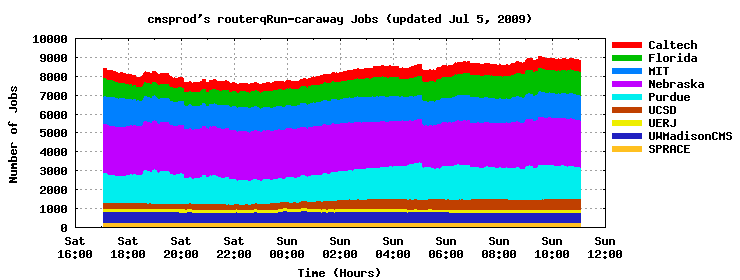
\includegraphics[height=4.5cm]{Graphics/routerqRun-caraway-Jul5.png}
    \caption{OSG production jobs, 4 - 5 July, 2009}
    \end{figure}
\end{frame}

\end{document}
